\chapter{Approach}
\label{cha:approach}
This chapter identifies the requirements a benchmark for time series forecasting need to fulfill to enable fair, accurate and reproducible comparisons. Furthermore, this chapter identifies assets and methods which need to be investigated further through experimental studies. In Chapter \ref{cha:designing}, these studies are performed. The concepts discussed in this chapter are in Chapter \ref{cha:crayon}, combined into Crayon, a benchmarking toolkit for forecasting methods which is used for the empirical comparison in Chapter \ref{cha:chapter6}.

\section{Defining Reproducibility}
In Section \ref{sec:reproducibility}, the term reproducibility was split into three categories; \textit{technical}, \textit{statistical} and \textit{conceptual}. A benchmarking toolkit should adhere to the requirements posed by these rules in order to be reproducible.

In addition to the requirements identified in Section \ref{sec:reproducibility}, automating the benchmark would lead to a higher degree of reproducibility as the benchmarks would be standardized and thus less error prone. However, certain aspects of a benchmark, such as the error metric, are not suitable to be standardized since suitable error metrics depends on the use case.

A summary of the requirements identified in this section for enabling reproducible benchmarks is presented below:

\begin{enumerate}
  \item Encapsulation tools shall be used for dependency and algorithm management.
  \item Experiments shall run multiple times in order to build up a distribution of errors such that the variance of the error is recorded.
  \item Statistical tests shall be applied to the results to enforce statistical reproducibility.
  \item Multiple datasets shall be used when benchmarking to cover various usecases for conceptual reproducibility.
  \item The benchmark shall be automated
\end{enumerate}


\section{Defining Fair Comparisons}
\label{sec:fair_comparisons}
The adjective Fair is defined as \textit{acceptable and appropriate in a particular situation.} in the Oxford Dictionary. When benchmarking forecasting models, one method of achieving fair comparisons is to evaluate algorithms on multiple complementary datasets as this showcases the strengths and weaknesses of algorithms in different scenarios. Additionally, fair comparisons also require that the variance is shown as this provides more detail of an algorithms overall performance than a single value \cite{bouthillier2021accounting}.

Simply executing an algorithm on multiple datasets is not enough as it is important to give each algorithm a fair opportunity to perform well on each dataset. This is normally achieved by \textit{tuning} the hyperparameters of an algorithm for the dataset in question. A fair way of tuning algorithms is however non trivial as different strategies tend to be biased \cite{sivaprasad2020optimizer}. One method of achieving fairness could be to limit the time spent for hyperparameter tuning to some constant value. This would however be unfair towards slower methods such as DNNs or RNNs as the search space traversed would be smaller when compared to faster models such as simple NNs or classical models. Another approach is to limit the size of the search space by limiting the number of hyperparameter configurations to be tested. This would benefit models with few hyperparameters as each hyperparameter would be more thoroughly tuned than if more hyperparameters would be available. The inverse of this would also hold, one could limit the number of configurations for each hyperparameter tested but let the total number of hyperparameter configurations to be unbound. This would however be unfair towards models with few parameters.

Another approach would be to tune each algorithm such that it achieves its \textit{optimal} performance for each dataset. This would be fair in the sense that it is independent of the complexity of the algorithm being tested. For ML competitions this is commonly the case as contestants tune their algorithms to perform optimally in order to win \cite{roelofs2019meta}. This is also the case when algorithms are used in practice as companies and organizations leveraging machine learning, spend considerable effort in tuning these to fit their data \cite{beam2020challenges}.

To enable fair comparisons the implementations of the models being compared should be bug-free and optimized. This is especially important for very complex models as the engineering effort of implementing such algorithms correctly is considerable.

A summary of the requirements for fair comparisons which have been identified are:

\begin{enumerate}
  \item Optimally tuned algorithms for each dataset
  \item Variance should be reported
  \item Models should be evaluated on multiple complementary datasets
  \item Reference implementations of tested forecasting models should be used when possible
\end{enumerate}

\section{Defining Accurate Comparisons}
In Section \ref{subsec:error_metrics}, different metrics were presented for comparing forecasting accuracy. It was established that error metrics have different strengths and weaknesses which makes different metrics suitable for different domains or applications.
Thus, in order to perform an accurate comparison of forecasting methods via a benchmarking system, multiple different metrics need to be made available.

\begin{figure}[htb]
  \centering
  \begin{subfigure}{0.47\textwidth}
    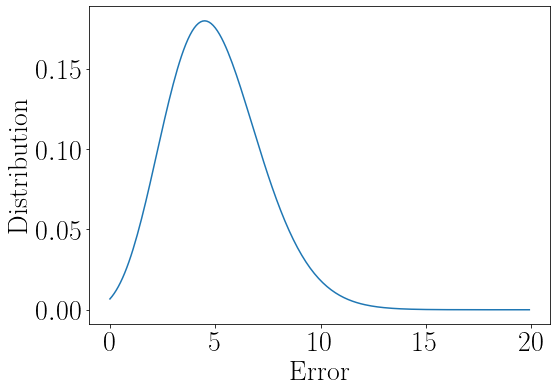
\includegraphics[width=\linewidth]{./img/poisson_distribution.png}
    \caption{Distribution far from 0}
    \label{fig:poisson}
  \end{subfigure}
  \hfill
  \begin{subfigure}{0.47\textwidth}
    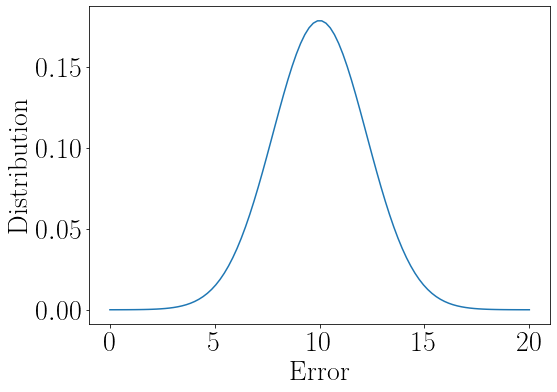
\includegraphics[width=\linewidth]{./img/normal_distribution.png}
    \caption{Distribution close to 0}
    \label{fig:normal}
  \end{subfigure}
  \hfill
  \caption{Two possible error distributions, the left one is more consistently close to zero and is thus better as an error of zero is desired.}
  \label{fig:example_distributions}
\end{figure}

Since, for reproducibility purposes, each model shall generate a distribution of error metrics one cannot any longer compare algorithms based on single metric values. Figure \ref{fig:example_distributions}, presents two examples of possible error distributions. Since a smaller error is generally considered better, it makes sense that distributions concentrated close to zero perform the best. For example, an algorithm generating an error distribution like in Figure \ref{fig:poisson}, is more likely to produce errors close to 0 than an algorithm producing the error distribution in Figure \ref{fig:normal}.

In summary to perform accurate comparisons:
\begin{enumerate}
  \item Suitable error metrics should be used for the domain and datasets.
  \item The distribution of the error metric over multiple runs shall be used when comparing different algorithms.
\end{enumerate}
